\section{The Intel 486}
Announced in 1989, the i486-25Mhz was a performance evolution which addressed all bottleneck of the 386 and shipped with an integrating FPU \footnote{Floating Point Unit}. Intel did not originally planned on two flavors (SX and DX) but manufacturing issues lead to producing 486 units with malfunctioning FPUs. Instead of throwing these away, Intel sold them at a discounted price. That is how PC builder could choose between a 486-SX and a 486-DX. In practice all video games used ony fixed point arithmetic, leaving the FPU unused. Therefore, a 486-SX offered the same performance as a 486-DX which made the former a good deal. Still, priced at \$950\footnote{\$950 is \$1,920 in 2017, adjusted to inflation.} for the DX 
and \$258\footnote{InfoWorld Apr 29, 1991.}\footnote{\$258 in 1991 is \$469.20 in 2017, adjusted to inflation.} for the SX, few could afford Intel's beast.\\
\par
On top of its price, the i486 had to face internal competition from an other CPU manufactured by Intel, the i860. The i860 relied on an heavily pipelined superscaler architecture crushing VLIWs\footnote{Very long instruction word.}. It three units, X, Y ,and Z allowed parallel processing which rendered it incompatible with the i386 instruction set. It heavily relied on compiler ability to 

\par
Checkout \cw{https://en.wikipedia.org/wiki/NEAT\_chipset} for details of motherboard.\\

Intel i860 vs Intel i486\\
\par
\fq{...We now had two very powerful chips that we were introducing at just about the same time: the 486, largely based on cisc technology and compatible with all the pc software, and the i860, based on risc technology, which was very fast but compatible with nothing. we didn't know what to do. so we introduced both, figuring we'd let the marketplace decide. however, things were not that simple. supporting a microprocessor architecture with all the necessary computer-related products --- software, sales, and technical support --- takes enormous resources. even a company like Intel had to strain to do an adequate job with just one architecture. and now we had two different and competing efforts, each demanding more and more internal resources. development projects have a tendency to want to grow like the proverbial mustard seed. the fight for resources and for marketing attention (for example, when meeting with the customer, which processor should we highlight) led to internal debates that were fierce enough to tear apart our microprocessor organization. meanwhile, our equivocation caused our customers to wonder what Intel really stood for, the 486 or i860?}{Andy Grove, "Only the paranoid survive".}
\par
\cfullimage{i860.png}{The Intel i860.}
\par
\cfullimage{i860_arch.png}{The Intel i860.}
\par
\cfullimage{i486DX.png}{The Intel 486 1.2 millions transistors.}
\par
Ultimately, the combined difficulty of the i860, the performance/backward compatibility, and Intel picking a favorite proved too much for the i860 to survive. For games it means studios were going to write games for DOS and the 486.

\trivia{Amusingly, the i860 would still play a part in Doom's development since it was used on NextDimension boards.}

\fq{Cray on a Chip\\
\par
The Intel 80860 was an impressive chip, able at top speed to perform close to 66 MFLOPS at 33 MHz in real applications, compared to a more typical 5 or 10 MFLOPS for other CPUs of the time. Much of this was marketing hype, and it never become popular, lagging behind most newer CPUs and Digital Signal Processors in performance.
The 860 has several modes, from regular scaler mode to a superscalar mode that executes two instructions per cycle and a user visible pipeline mode (instructions using the result register of a multi-cycle op would take the current value instead of stalling and waiting for the result). It can use the 8K data cache in a limited way as a small vector register (like those in supercomputers). The unusual cache uses virtual addresses, instead of physical, so the cache has to be flushed any time the page tables changes, even if the data is unchanged. Instruction and data busses are separate, with 4 G of memory, using segments. It also includes a Memory Management Unit for virtual storage.\\
\par
The 860 has thirty two 32 bit registers and thirty two 32 bit (or sixteen 64 bit) floating point registers. It was one of the first microprocessors to contains not only an FPU as well as an integer ALU, and also included a 3-D graphics unit (attached to the FPU) that supports lines drawing, Gouraud shading, Z-buffering for hidden line removal, and operations in conjunction with the FPU. It was also the first able to do an integer operation, and a (unique at the time) multiply and add floating point instruction, for the equivalent of three instructions, at the same time.\\
\par
However actually getting the chip at top speed usually requires using assembly language - using standard compilers gives it a speed closer to other processors. Because of this, it was used as a coprocessor, either for graphics, or floating point acceleration, like add in parallel units for workstations. Another problem with using the Intel 860 as a general purpose CPU is the difficulty handling interrupts. It is extensively pipelined, having as many as four pipes operating at once, and when an interrupt occurs, the pipes can spill and lose data unless complex code is used to clean up. Delays range from 62 cycles (best case) to 50 microseconds (almost 2000 cycles).}{John Bayko, University of Regina}

\subsection{Floating Point Unit}
The i386 was able to talk to an i387 located on the motherboard. Requests and responses had to transition on the bus and incurred four CPU cycles of overhead. For the i486, Intel decided to integrate the i487 FPU in the same die and improved performance by a factor 2.\\
\par
TODO: Drawing
\par

TODO: Verify with 387/487 description




\par
\begin{figure}[H]
\centering
\begin{tabularx}{\textwidth}{ X  X X  X  X}
  \toprule
  \textbf{CPU} & \textbf{FADD} & \textbf{FMUL} & \textbf{FDIV} &\textbf{FXCH} \\ \bottomrule
Intel 387 & 23-34 & 29-57   & 88-91 & 18 \\
Intel 487 & 8-20  & 16   & 73 & 4 \\ \bottomrule
\end{tabularx}
\caption{FPU performance: 387 vs 487.}
\label{perf_summary}
\end{figure}

\subsection{Pipeline}



\begin{figure}[H]
\centering
\includegraphics[width=\textwidth]{drawings/386_instruction_pipeline.pdf}
\caption{386 pipeline in Intel documentation.}
\end{figure}
\par


\begin{figure}[H]
\centering
\includegraphics[width=\textwidth]{drawings/actual_386_instruction_pipeline.pdf}
\caption{386 pipeline: Two cycles per instruction.}
\end{figure}
\par

\begin{figure}[H]
\centering
\includegraphics[width=\textwidth]{drawings/actual_486_instruction_pipeline.pdf}
\caption{486 pipeline: One cycle per instruction.}
\end{figure}
\par

\subsection{Cache L1}
four-way set-associative write through.\\

\subsection{Cache L2}
Bla
\subsection{Precaching (cachelines) Netburst}
Bla


\begin{figure}[H]
\centering
\scaledimage{0.9}{486_blueprint.png}
\end{figure}
\par
\begin{figure}[H]
\centering
\scaledimage{0.9}{486_layout.png}
\end{figure}








\section{Overdrive, 486 DX2 66Mhz}
\begin{figure}[H]
\centering
  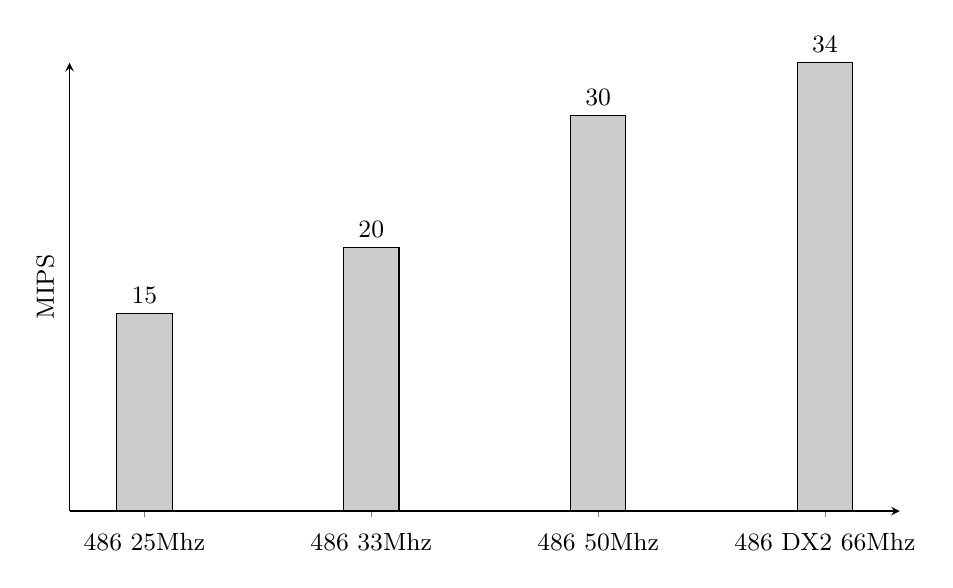
\begin{tikzpicture}[font=\small]
    \begin{axis}[
      width=1.0\textwidth,
      height=0.6\textwidth,
      ybar,
      bar width=20pt,
      ylabel={MIPS},
      ymin=0,
      ytick=\empty,
      xtick=data,
      axis x line=bottom,
      axis y line=left,
      enlarge x limits=0.11,
      symbolic x coords={486 25Mhz,486 33Mhz,486 50Mhz,486 DX2 66Mhz},
      xticklabel style={anchor=base,yshift=-\baselineskip},
      nodes near coords={\pgfmathprintnumber\pgfplotspointmeta}
    ]
      \addplot[fill=black!20,draw=black] coordinates {
        (486 25Mhz,15)
        (486 33Mhz,20)
        (486 50Mhz,30)
        (486 DX2 66Mhz,34)
      };
    \end{axis}
   
   \end{tikzpicture}
   \caption{Comparison\protect\footnotemark of CPUs with MIPS \protect\footnotemark.}
 \end{figure}
\footnotetext{Source: "Roy Longbottom's PC Benchmark Collection: http://www.roylongbottom.org.uk/mips.htm".}

Zero-wait state.\\
DRAM vs SRAM\\
Cache hit percentage from ISA book.\\
four-way set-associative write back.\\


\subsection{Performance \& Price}
By may 1992, the Intel 386 was being replaced by a new version, the 486. The increase in operatin frequency was substancial for the high end model running at 50Mhz but most 486 ran at the same speed at the 386: 25Mhz and 33Mhz. The revolutionary design of the CPU.\\

\par
\begin{figure}[H]
\centering
  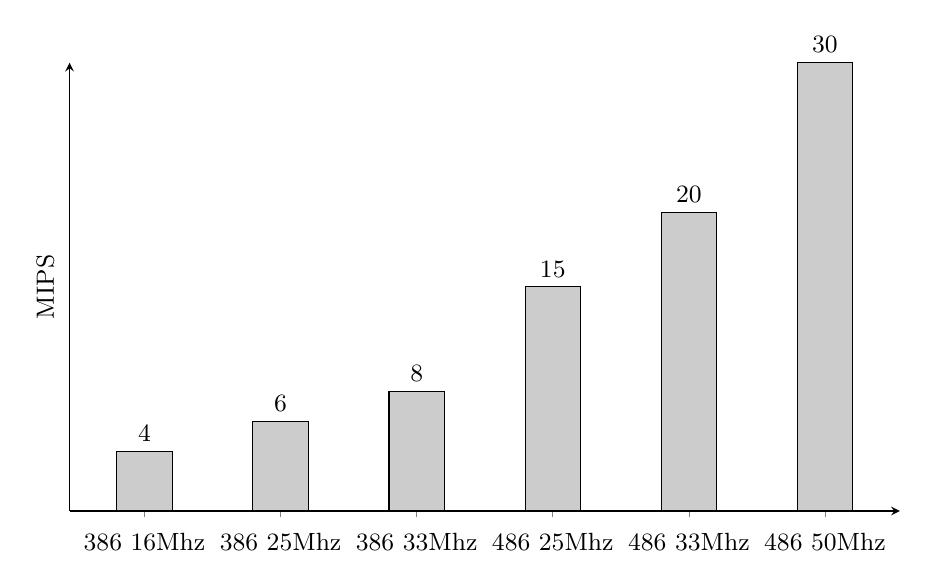
\begin{tikzpicture}[font=\small]
    \begin{axis}[
      width=1.0\textwidth,
      height=0.6\textwidth,
      ybar,
      bar width=20pt,
      ylabel={MIPS},
      ymin=0,
      ytick=\empty,
      xtick=data,
      axis x line=bottom,
      axis y line=left,
      enlarge x limits=0.11,
      symbolic x coords={386 16Mhz,386 25Mhz,386 33Mhz,486 25Mhz,486 33Mhz,486 50Mhz},
      xticklabel style={anchor=base,yshift=-\baselineskip},
      nodes near coords={\pgfmathprintnumber\pgfplotspointmeta}
    ]
      \addplot[fill=black!20,draw=black] coordinates {
        (386 16Mhz,4)
        (386 25Mhz,6)
        (386 33Mhz,8)
        (486 25Mhz,15)
        (486 33Mhz,20)
        (486 50Mhz,30)
      };
    \end{axis}
   
   \end{tikzpicture}
   \caption{Comparison\protect\footnotemark of CPUs with MIPS \protect\footnotemark.}
 \end{figure}
\footnotetext{Source: "Roy Longbottom's PC Benchmark Collection: http://www.roylongbottom.org.uk/mips.htm".}